%%%%%%%%%%%%%%%%%%%%%%%%%%%%%%%%%%%%%%%%%%%%%
% Laatste aanpassingen:  
% sept 2013 [Jan]: deel log. vgl uitgecommentarieerd
%                   
%  11/09/2012 [Greetje] herwerkt: verdubbelingstijd als oefening op logaritmen naar dit hoofdstuk gebracht omdat de hoofdstukken groei en exp functie omgewisseld zijn in de cursus.
% 14/02/11 [Greetje]: hoofdstuk herwerkt
% 19/9/02 [Jan]: dubbel label veranderd (tbl:logexpverband)
%                 
% 9/9/02 [Jan]: figuren in aparte map. Verwijzingen naar Mathcad
%    weggewerkt.
%                       
% 04/08/02 door Roby                        
%      tekeningen aangepast aan Euler    
%    
% 10/09/01 door Greetje                     
%   typfouten van Roby                      
%   lay-out van titels (ihb boldmath)  
%     
% 01/09/01 door Greetje                     
%%%%%%%%%%%%%%%%%%%%%%%%%%%%%%%%%%%%%%%%%%%%%


\chapter{Exponenti\"ele en logaritmische functies}
\label{chap:expFunctie}


\begin{quote}
     \textit{ `Kun jij optellen?' vroeg de Witte Koningin.
     `Wat is \'{e}\'{e}n en \'{e}\'{e}n en \'{e}\'{e}n en \'{e}\'{e}n
     en \'{e}\'{e}n en \'{e}\'{e}n en \'{e}\'{e}n en \'{e}\'{e}n en
     \'{e}\'{e}n en \'{e}\'{e}n en \'{e}\'{e}n en \'{e}\'{e}n?'}

     \textit{`Weet ik niet,' zei Alice, `ik ben de tel kwijt.'}

     \textit{`Optellen kan ze niet,' onderbrak de Rode Koningin. `Kun je
          aftrekken? Trek negen af van acht.'}

     \textit{`Acht min negen kan ik niet, hoor,' antwoordde Alice zeer
          bereidwillig, `maar--'}

     \textit{`Aftellen kan ze niet,' zei de Witte Koningin. `Kun je delen? Een
          brood gedeeld door een mes -- wat is \emph{dat}?'}

          Uit `Achter de spiegel' -- Lewis Carroll
\end{quote}


\newpage
\section{Inleiding}
In \cref{chap:groei} introduceerden we het begrip `exponentiële groei'. In dit hoofdstuk veralgemenen we dit begrip tot exponentiële functies. Waar we tot nog toe rekening hielden met de beginwaarde $B(0)$, beperken we ons in wat volgt tot functies van de vorm $B(x)=g^x$. 

Bij een groeiproces stelden we ons enkel de vraag `hoeveel algen zijn er na 3 weken'. De vraag `wanneer is de vijver volgroeid' konden we nog niet exact beantwoorden, we waren tevreden met een numerieke benadering. Voor de exacte oplossing hebben we de logaritmische functie nodig. Dit behandelen we in het tweede deel van dit hoofdstuk.

\section{ Exponenti\"{e}le functie}\label{sec.expfunctie}
\subsection{Macht met re\"ele exponent}\label{subsec:macht}
In dit hoofdstuk hebben we machten van getallen nodig. We willen \emph{elke} macht van een gegeven getal berekenen. Maar hoe bereken je bijvoorbeeld $2^{\sqrt 2}$? We verduidelijken dit in deze sectie.

De eenvoudigste groep machten zijn die  met een rationale exponent (gehele getallen en breuken).
Dit `soort' machten krijgt betekenis door gebruik te maken van
producten, delingen en worteltrekkingen. We nemen als voorbeeld machten met grondtal~$2$:

\begin{displaymath}
    2^{4}=2\cdot 2\cdot 2\cdot 2
\end{displaymath}
\begin{displaymath}
    2^{-2}=\frac{1}{2^{2}}=\frac{1}{4}
\end{displaymath}
\begin{displaymath}
    2^{\frac{3}{2}}=\sqrt{2^{3}}
\end{displaymath}

Machten met een re\"ele exponent die \emph{geen} rationaal getal zijn (getallen die je niet als breuk kan schrijven, bijvoorbeeld $\pi$ en  $\sqrt{2}$) kunnen we op die manier niet berekenen.
In wat volgt laten we zien hoe we deze groep van machten zoals $2^{\pi}$ of $7^{\sqrt{2}}$ wel kunnen bepalen.
Als voorbeeld nemen we $2^{\pi}$.

We zoeken een rij van \emph{rationale getallen} die $\pi$ steeds dichter
benaderen.
Aangezien $\pi=\num{3.141592654}$\dots\ kunnen we de rij starten met $\num{3.1}$,
en verder telkens een decimaal meer nemen om de benadering beter te
maken. We noemen de rij getallen $t_{i}$. In \cref{tbl:pibenadering}
zijn deze getallen gegeven en
berekenen we de respectievelijke machten van 2.

\begin{table}[!h]
    \centering
    \caption{Benadering van $2^{\pi}$ }
    \begin{tabular}{cSS}
    \toprule
    $i$ & $t_{i}$ & ${2^{t_{i}}}$  \\
    \midrule
    1 & 3.1 & 8.574188  \\
    2 & 3.14 & 8.815241  \\
    3 & 3.141 & 8.821353  \\
    4 & 3.1415 & 8.824411  \\
    5 & 3.14159 & 8.824962  \\
    6 & 3.141592 & 8.824974  \\
    \bottomrule
\end{tabular}  \\
    \label{tbl:pibenadering}
\end{table}
 De rij getallen $2^{t_{i}}$ nadert naar een getal, waarvan we
 voorlopig alleen de eerste decimalen kennen, nl \num{8.8249}. Willen we
 meer decimalen van dit getal kennen, dan moeten we meer elementen van de rij
 berekenen.
Het getal, waarnaar de rij getallen $2^{t_{i}}$ evolueert,
 stellen we gelijk aan $2^{\pi}$. 

 \begin{displaymath}
     2^{\pi}=\lim_{t_{i}\rightarrow \pi}2^{t_{i}}
 \end{displaymath}
 Voor de andere irrationale getallen kunnen we een gelijkaardige  benadering maken. 

\subsection{Exponenti\"{e}le functie}
Naar analogie met vergelijking~\eqref{eq:eq_groei2} definiëren we de exponentiële functie als volgt:
\begin{quote}
De functie 
\begin{equation}
y=g^x 
\label{eq:def_exp_func}
\end{equation}
noemen we de \emph{exponenti\"ele functie}\index{exponenti\"ele functie} met \emph{grondtal}\index{grondtal} $g$. De onafhankelijk veranderlijke $x$  noemen we de \emph{exponent}\index{exponent}.
Het domein van de functie is $\real$.
\end{quote}
De nieuwe functie $f(x)=g^{x}$ noemen we \emph{exponentieel}, omdat de
onafhankelijk veranderlijke $x$ in de \emph{exponent} staat.

In \cref{fig:2x} vind je de grafiek van $2^{x}$. De benadering van bijvoorbeeld $2^\pi$ die we maakten in \cref{subsec:macht} krijgt op deze manier een grafische betekenis: de `gaten', die er
 in irrationale punten van de grafiek nog waren, zijn opgevuld tot een vloeiende kromme.

 \begin{figure}[htbp]
      \centering
     \begin{tikzpicture}[line cap=round,line join=round,x=1.0cm,y=0.2cm]
\draw[->] (-2.2,0) -- (5.5,0) node [at end, below] {$x$};
\foreach \x in {-2,...,5}
\draw[shift={(\x,0)}] (0pt,2pt) -- (0pt,-2pt) node[below] {\footnotesize $\x$};
\draw[->] (0,0) -- (0,35) node [at end, left] {$y$};
\foreach \y in {5,10,...,30}
\draw[shift={(0,\y)},color=black] (2pt,0pt) -- (-2pt,0pt) node[left] {\footnotesize $\y$};
\draw [domain=-2:5,thick] plot(\x,{exp(\x*ln(2))});
\draw [dashed, gray] (2,0) |- (0,4);
\draw [dashed, gray] (3,0) |- (0,8);
    \filldraw [blue] (2,4) circle (2pt);
        \filldraw [blue] (3,8) circle (2pt);
\end{tikzpicture}
     \caption{Grafiek van $2^{x}$}
     \label{fig:2x}
 \end{figure}

Voor een functie is het belangrijk dat het beeld voor alle $x$-waarden van het domein, op een beperkt aantal uitzonderingen na, berekend kan worden (de functie moet `overal gedefinieerd' zijn). Daardoor is het grondtal $g$ zoals gedefinieerd in \eqref{eq:def_exp_func} onderworpen aan een aantal voorwaarden.
\begin{description}
\item[ Het grondtal moet positief zijn]  
Neem bijvoorbeeld $g=-2$. Dan kan je $g^x$ voor heel wat getallen niet berekenen: bijvoorbeeld $(-2)^\frac12=\sqrt{-2}$ bestaat niet.
\item[Het grondtal moet verschillend van $0$ zijn] want $0^{x}$ bestaat
    niet als $x\leq 0$. Bijvoorbeeld  voor $g=0$ en $x=-1$ zouden we $0^{-1}=\frac{1}{0}$ moeten berekenen, en dat quoti\"ent bestaat niet.
\item[Het grondtal moet verschillend zijn van 1] De functie $y=1^x$ bestaat en is overal gedefinieerd. Omdat $1^x=1$ voor elke $x$ is deze functie een constante functie en vertoont ze geen `groei'. Daardoor heeft deze functie een ander `karakter' dan exponenti\"ele functies met een ander grondtal en beschouwen we $y=1^x$ \emph{niet} als exponenti\"ele functie.
\end{description}

In de volgende secties bespreken we het verloop van de grafiek van de exponenti\"ele functie in detail. We onderscheiden hierbij twee gevallen, namelijk $g>1$ en $0<g<1$.

\subsection[Eigenschappen van de exponenti\"{e}le functie met
$g>1$]{Eigenschappen van de exponenti\"{e}le functie met \boldmath
$g>1$\unboldmath}\label{subsec.ggroter1}
 \begin{figure}[htbp]
      \centering
          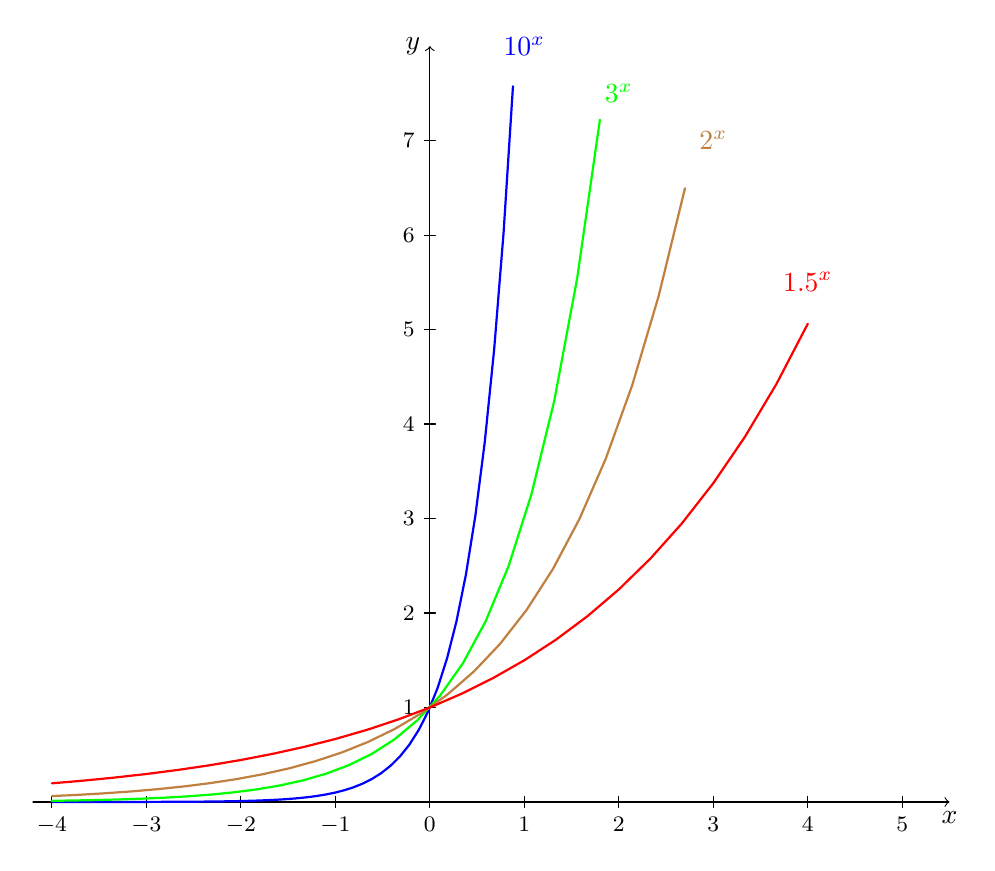
\begin{tikzpicture}[line cap=round,line join=round,x=1.2cm,y=1.2cm]
\draw[->] (-4.2,0) -- (5.5,0) node [at end, below] {$x$};
\foreach \x in {-4,...,5}
\draw[shift={(\x,0)}] (0pt,2pt) -- (0pt,-2pt) node[below] {\footnotesize $\x$};
\draw[->] (0,0) -- (0,8) node [at end, left] {$y$};
\foreach \y in {1,...,7}
\draw[shift={(0,\y)},color=black] (2pt,0pt) -- (-2pt,0pt) node[left] {\footnotesize $\y$};
\draw [domain=-4:0.88,samples=50,thick,blue] plot(\x,{exp(\x*ln(10))}); \draw[blue] (1,8) node {$10^x$};
\draw [domain=-4:1.8,thick,green] plot(\x,{exp(\x*ln(3))});
\draw[green] (2,7.5) node {$3^x$};
\draw [domain=-4:2.7,thick,brown] plot(\x,{exp(\x*ln(2))});
\draw[brown] (3,7) node {$2^x$};
\draw [domain=-4:4,thick,red] plot(\x,{exp(\x*ln(1.5))});
\draw[red] (4,5.5) node {$\num{1.5}^x$};
\end{tikzpicture}
     \caption{Grafiek van $\num{1.5}^{x};~2^x;~3^x$ en $10^x$}
     \label{fig:groter1}
 \end{figure}

In \cref{fig:groter1} worden de exponenti\"ele functies $f(x)=g^x$ met grondtal $g$ gelijk aan $\num{1.5}$; $2$; $3$ en $10$ getekend. Elke functie vertoont volgende eigenschappen: 
\begin{enumerate}
    \item  Het domein van de hierboven vermelde functies is steeds $\real$, de re\"{e}le
    getallenverzameling.
    \[
      \dom{f}=\real
    \]

    \item  Omdat $g^x>0$ als $g>0$ bestaat het bereik of het beeld (projectie van de functie op de $y$-as) uit alle strikt positieve re\"{e}le getallen. 
    \[
      \range{f}=\real^+_0=\{x|x\in \real \text{~en~} x>0\}
    \]
    
    \item Om die reden is er ook \emph{geen snijpunt} met de $x$-as. De functies hebben  geen nulpunt.

    \item  Het snijpunt met de $y$-as is het punt (0,1).

  
    \item  \label{exp_func:inject} De functies zijn \emph{injectief} (\cref{subsec:jectief}, pagina~\pageref{subsec:jectief}). Dit betekent dat bij iedere $x$-waarde een verschillende $y$-waarde hoort. Anders gezegd: twee
    functiewaarden  kunnen nooit aan elkaar gelijk zijn  voor
    verschillende waarden van $x$. 
        \begin{displaymath}
        g^{x_{1}}=g^{x_{2}}   \; \Leftrightarrow \; x_{1}=x_{2}
    \end{displaymath}
    Dit is belangrijk als we de inverse functie willen bepalen.
    
    \item  De functies zijn  \emph{strikt stijgend} op het domein en
    hebben geen maximum.

    \item  Voor \emph{grote negatieve waarden} van $x$ gaan de functiewaarden naar 0.
    \[
    \lim_{x\rightarrow-\infty}f(x)=0
    \]

\end{enumerate}
Als we de functies met verschillend grondtal vergelijken, merken we dat de \emph{functie sneller stijgt naargelang het grondtal groter wordt}. 
\begin{itemize}
\item voor positieve $x$-waarden wordt de functiewaarde sneller groter als $x$ groter wordt;
\item voor negatieve $x$-waarden daalt de functiewaarde sneller (gaat de functiewaarde sneller naar $0$) als  $x$ kleiner wordt (als $x$ meer negatief wordt).
\end{itemize}




\subsection[Eigenschappen van de exponenti\"{e}le functie met $g<1$]{Eigenschappen van de exponenti\"{e}le functie met \boldmath$0<g<1$\unboldmath}
In \cref{tab:expfunckleiner1} lijsten we een aantal functiewaarden op van de functies $f(x)=2^x$ en $h(x)=\left(\frac12\right)^x$.
%\renewcommand{\tabcolsep}{0.5cm}
%\renewcommand{\arraystretch}{2}
\begin{table}[htdp]
\caption{Functiewaarden van de functies $f(x)=2^x$ en $h(x)=\left(\frac12\right)^x$}
\centering
\begin{tabular}{c|ccccccc}
$x$&$-3$&$-2$&$-1$&0&1&2&3\\ 
\midrule
$f(x)=2^x$&$\frac18$&$\frac14$&$\frac12$&1&2&4&8\\
$h(x)=\left(\frac12\right)^x$&8&4&2&1&$\frac12$&$\frac14$&$\frac18$
\end{tabular}
\label{tab:expfunckleiner1}
\end{table}%

Je merkt dat $f(-x)=h(x)$ 
\begin{displaymath}
    f(-x)=2^{-x}=\frac{1}{2^{x}} =\left(\frac{1}{2}\right)^{x}
\end{displaymath}
Beide functies zijn mekaars \emph{spiegelbeeld ten opzichte van de $y$-as}. Dit blijkt ook uit \cref{fig:1/2x}.
\begin{figure}[htbp]
    \centering
        \begin{tikzpicture}[line cap=round,line join=round,x=1.0cm,y=0.5cm]
\draw[->] (-4.2,0) -- (4.5,0) node [at end, below] {$x$};
\foreach \x in {-4,...,4}
\draw[shift={(\x,0)}] (0pt,2pt) -- (0pt,-2pt) node[below] {\footnotesize $\x$};
\draw[->] (0,0) -- (0,17.5) node [at end, left] {$y$};
\foreach \y in {2,4,...,16}
\draw[shift={(0,\y)},color=black] (2pt,0pt) -- (-2pt,0pt) node[left] {\footnotesize $\y$};
\draw [domain=-4:4,thick,blue] plot(\x,{exp(\x*ln(2))});
\draw[blue] (4,16.5) node {$f(x)=2^x$};
\draw [domain=-4:4,thick,red] plot(\x,{exp(\x*ln(0.5))});
\draw[red] (-4,16.8) node {$h(x)={(\frac{1}{2})}^x$};
\draw [dashed, gray] (2,0) |- (0,4);
\draw [dashed, gray] (-2,0) |- (0,4);
    \filldraw [blue] (2,4) circle (2pt);
        \filldraw [red] (-2,4) circle (2pt);
\end{tikzpicture}
    \caption{Grafieken van $f(x)=2^{x}$ en $h(x)={(\frac{1}{2})}^{x}$}
    \label{fig:1/2x}
\end{figure}
Uit deze figuur blijkt ook dat de eigenschappen 1 tot en met 5 die opgesomd werden in \cref{subsec.ggroter1} behouden blijven. In tegenstelling met de exponenti\"ele functie met $g>1$, is de exponenti\"ele functie met grondtal kleiner dan 1 \emph{dalend}. Voor grote  positieve waarden van $x$ gaan de functiewaarden naar~0.
\[
\lim_{x\rightarrow+\infty}h(x)=0
\]


 \subsection{Opmerkingen}
 \begin{enumerate}
     \item  De machtsfunctie $y=x^{5}$ en de exponenti\"{e}le functie
     $y=5^{x}$ verschillen grondig van elkaar. Bij een \emph{machtsfunctie}\index{machtsfunctie}
     is het grondtal de onafhankelijk veranderlijke en kan je de
     functiewaarden berekenen via \\$x^{5}=x\cdot x\cdot x\cdot x\cdot x$. Bij de
     \emph{exponenti\"{e}le functie} staat de onafhankelijk veranderlijke in
     de exponent en moet je de functiewaarde berekenen zoals uitgelegd in \cref{subsec:macht}.

     \item  Bij de exponenti\"{e}le functies gelden dezelfde
     \emph{rekenregels} als bij de machtsfuncties:
     \begin{align*}
       g^{x+y} & =g^{x}\cdot g^{y} \\
       \left(g^{x}\right)^{y} & =\left(g^{y}\right)^{x}=g^{x\cdot y} \\
       g^{-x} & =\frac{1}{g^{x}}
     \end{align*}
 \end{enumerate}



\section{Logaritmische functie}
\subsection{Inleiding}
We beginnen deze sectie met een voorbeeld. 
\begin{quote}
Neem een lint van \SI{1}{\meter}. Vouw dat een aantal keren in twee. Het geplooide
lint wordt telkens de helft korter.
\begin{itemize}
    \item  Na hoeveel keren plooien is de lengte van het geplooide lint gelijk aan \SI{1/8}{\meter}?

    \item  Na hoeveel keren plooien is de lengte kleiner dan \SI{1/100}{\meter}?
\end{itemize}
\end{quote}
Het antwoord op de eerste vraag zoeken we met proberen. Na \'e\'en keer plooien is de lengte van het lint gehalveerd, na twee keer plooien is de lengte nog maar een vierde van zijn oorspronkelijke lengte en na drie keer plooien is de lengte \'e\'en achtste van een meter lang. De lengte van het lint moet dus drie keer gehalveerd worden.  Merk op dat  $\frac18=\left(\frac12\right)^3$. Het getal 3 (het aantal keren plooien) is de exponent die we aan $\frac12$ (de factor waarmee het lint ingekort wordt) moeten geven om $\frac18$ (de lengte van het geplooide lint) te bekomen.

Voor de  tweede vraag moeten we dus het volgend probleem oplossen: zoek de
exponent die je aan $\frac{1}{2}$ moet geven om $\frac{1}{100}$ te
bekomen. In termen van de exponenti\"{e}le functie betekent dit:
zoek $x$ zodat $\left(\frac{1}{2}\right)^{x}=\frac{1}{100}$. We zoeken de exponent terwijl de functiewaarde gekend is. Dit
kennen we als het bepalen van de inverse van de exponenti\"{e}le functie. Deze inverse
functie noemen we de \emph{logaritmische functie met grondtal
$\frac{1}{2}$}\index{logaritme}. Mits wat geduldig blijven delen door 2 vinden we als
antwoord $7$ want $\left(\frac{1}{2}\right)^{7}<\frac{1}{100}$.

\subsection[Definitie van de logaritmische functie $\log_{g}$]
{Definitie van de logaritmische functie
\boldmath$\log_{g}$\unboldmath}
\begin{quote}
   De inverse functie  van de exponenti\"ele 
functie $y=g^{x}$ noemen we de \emph{logaritmische functie met grondtal g}.
\[
y=\log_{g}(x)
\]
\end{quote}
In \cref{sec:invrelatie} definieerden we de inverse relatie door bron- en doelverzameling met mekaar te verwisselen: je moet dus $x$ en $y$ `met mekaar verwisselen'. 
Neem bijvoorbeeld $y=2^x$. De functie $y=2^x$ definieert voor elke $x$ uit het domein een beeld $y$. Om de inverse functie te bepalen moet je dat omkeren en zoeken welke $x$-waarde hoort bij een gegeven $y$. Kies een $y$-waarde, bijvoorbeeld $y=8$. Ga op \cref{fig:2x} vanuit het punt $(0,8)$ naar rechts totdat je de kromme van de functie tegenkomt. Ga vervolgens naar beneden totdat je de $x$-as tegenkomt. De $x$-waarde waar je de $x$-as bereikt (hier $x=3$) is de inverse functiewaarde van $y=8$. 

Als de functie voorgesteld wordt met behulp van een grafiek, vind je de grafische voorstelling van de inverse functie door haar te spiegelen ten opzichte van de bissectrice van het eerste kwadrant (dit is de rechte $y=x$).  De grafiek van $\log_{g}$ vinden we dus door de grafiek van $g^{x}$ te spiegelen ten opzichte van de bissectrice van het
eerste kwadrant. In \cref{fig:log2} tonen we de functies $f(x)=2^x$ en $k(x)=\log_2x$.

\begin{figure}[htbp]
    \centering
        \begin{tikzpicture}[line cap=round,line join=round,x=0.8cm,y=0.8cm]
\draw[->] (-3.2,0) -- (8.5,0) node [at end, below] {$x$};
\foreach \x in {-3,...,-1,1,2,...,8}
\draw[shift={(\x,0)}] (0pt,2pt) -- (0pt,-2pt) node[below] {\footnotesize $\x$};
\draw[->] (0,-3.2) -- (0,8.5) node [at end, left] {$y$};
\foreach \y in {-3,-2,-1,1,2,...,8}
\draw[shift={(0,\y)},color=black] (2pt,0pt) -- (-2pt,0pt) node[left] {\footnotesize $\y$};
\node[below left] (0,0) {\footnotesize $0$};
\draw [domain=-3:3.1,thick] plot(\x,{exp(\x*ln(2))});
\draw [dashed, gray] (3,0) |- (0,8);
\filldraw [blue] (3,8) circle (2pt);
\draw[] (2,6) node {$2^x$};
\draw [domain=0.1:8.4,samples=80,thick] plot(\x,{ln(\x)/ln(2)});
\draw [dashed, gray] (8,0) |- (0,3);
\filldraw [blue] (8,3) circle (2pt);
\draw[] (6,2) node {$\log_2(x)$};
\end{tikzpicture}
    \caption{Grafieken van $2^{x}$ en $\log_{2}(x)$}
    \label{fig:log2}
\end{figure}

Enkele belangrijke logaritmische functies zijn:
\begin{eqnarray*}
    \log_{10}(x) & = & \log(x)  \\
    \log_{e}(x) & = & \ln(x) \\
     \end{eqnarray*}
met  $e=\num{2.1828}\ldots$ (het getal van Euler). \\

Uit de definitie leiden we onmiddellijk volgend verband af:
\begin{displaymath}
    \log_{g}(x)=y   \Leftrightarrow  g^{y}=x
\end{displaymath}
We verwoorden als volgt: De logaritme $\log_{g}(x)$ is de
exponent $y$ die we aan het grondtal $g$ moeten geven om $ x$ te
bekomen.






Hieruit volgt:
\begin{eqnarray*}
    \log_{2}8=3 & \mbox{want} & 2^{3}=8  \\
    \log_{2}\left(\frac{1}{4}\right)=-2 & \mbox{want} & 2^{-2}=\frac{1}{4}  \\
    \log_{2}(\sqrt{2})=\frac{1}{2} & \mbox{want} &  2^{\frac{1}{2}}=\sqrt{2}
\end{eqnarray*}

Aangezien de logaritmische functie de inverse is van de
exponenti\"{e}le functie, geldt opnieuw dat de functie niet
gedefinieerd is voor $g\leq 0$ en $g=1$.  

Voor het verloop van de logaritmische functie maken
we, net zoals in \cref{sec.expfunctie}, een onderscheid
tussen $g>1$ en $0<g<1$.

\subsection[Verloop van de logaritmische functie met $g>1$]
{Verloop van de logaritmische functie met
\boldmath$g>1$\unboldmath} \label{sec:logfuncgroter1}

\begin{figure}[htbp]
    \centering
        \begin{tikzpicture}[line cap=round,line join=round,x=1cm,y=0.8cm]
\draw[->] (-0.2,0) -- (11,0) node [at end, below] {$x$};
\foreach \x in {1,...,10}
\draw[shift={(\x,0)}] (0pt,2pt) -- (0pt,-2pt) node[below] {\footnotesize $\x$};
\draw[->] (0,-5) -- (0,6) node [at end, left] {$y$};
\foreach \y in {-4,...,-1,1,2,...,5}
\draw[shift={(0,\y)},color=black] (2pt,0pt) -- (-2pt,0pt) node[left] {\footnotesize $\y$};
\node[below left] (0,0) {\footnotesize $0$};
\draw [domain=0.15:9,samples=80,thick,blue] plot(\x,{ln(\x)/ln(1.5)});
\draw[blue] (10,5.5) node {$\log_{\num{1,5}}(x)$};
\draw [domain=0.02:9,samples=100,thick,green] plot(\x,{ln(\x)/ln(3)});
\draw[green] (10,2) node {$\log_{\num{3}}(x)$};
\draw [domain=0.001:9,samples=100,thick,red] plot(\x,{ln(\x)/ln(10)});
\draw[red] (10,0.8) node {$\log_{\num{10}}(x)$};
\end{tikzpicture}
    \caption{Grafieken van $\log_{1.5}x$, $\log_3x$ en $\log_{10}x$}
    \label{fig:loggroter1}
\end{figure}
We leiden de eigenschappen af uit \cref{fig:loggroter1}.
\begin{enumerate}
     \item  Het \emph{domein} van de logaritmische functie is de verzameling van alle
    positieve re\"{e}le getallen. 
    \[
      \dom{\log_g(x)}=\real^{+}_{0}
    \]

    \item  Het bereik van de functie is $\real$. 
    \[
      \range{\log_g(x)}=\real
    \]
   \item  Alle grafieken gaan door het punt (1,0): 1 is het \emph{nulpunt}
    van de logaritmische functie.

    \item  De functie is  één-op-één of \emph{injectief} (verschillende $x$-waarden hebben verschillende $y$-waarden).
    \item  De logaritmische functie met grondtal $g$ groter dan 1 is \emph{stijgend} op haar domein. Ze heeft geen maximum.


    \item  Als $x$ nadert naar 0 dan worden de functiewaarden erg negatief. Voor grote (positieve) waarden van $x$ wordt de functiewaarde ook erg groot.
    \[
    \lim_{x\rightarrow0}\log_g(x)=-\infty \qquad \lim_{x\rightarrow+\infty}\log_g(x)=+\infty
    \]
\end{enumerate}

Als je in \cref{fig:loggroter1} de verschillende functies met mekaar vergelijkt, dan merk je dat de grafiek meer tegen de $x$-as `aanhurkt' naarmate het grondtal groter is. Als het grondtal $g$ groot is, verandert de macht $y=g^x$ snel als de exponent $x$ een klein beetje verandert. 

\subsection[Verloop van de logaritmische functie met
$0<g<1$] {Verloop van de logaritmische functie met
\boldmath$0<g<1$\unboldmath} 

\cref{fig:log1/2} toont de
logaritmische functie voor grondtal $g=\frac{1}{2}$ als inverse van de functie $y=\left(\frac12\right)^x$. 
In \cref{fig:loggroterkleiner} worden de functies $y=\log_2x$ en $y=\log_{\frac12}x$ getoond. Zoals de grafieken van de exponenti\"ele functies $y=2^x$ en $y=\left(\frac12\right)^x$ mekaars spiegelbeeld waren ten opzichte van de $y$-as, merken we nu dat de grafieken van de logaritmische functies  $y=\log_2x$ en $y=\log_{\frac12}x$ mekaars spiegelbeeld zijn ten opzichte van de $x$-as. 

De eigenschappen 1 t.e.m.\  4 zoals beschreven in \cref{sec:logfuncgroter1} blijven behouden. Het belangrijkste verschil met  de logaritmische functies met $g>1$ bestaat erin dat  de functies nu dalend zijn en overgaan van positief naar negatief:
\begin{figure}[htbp]
    \centering
        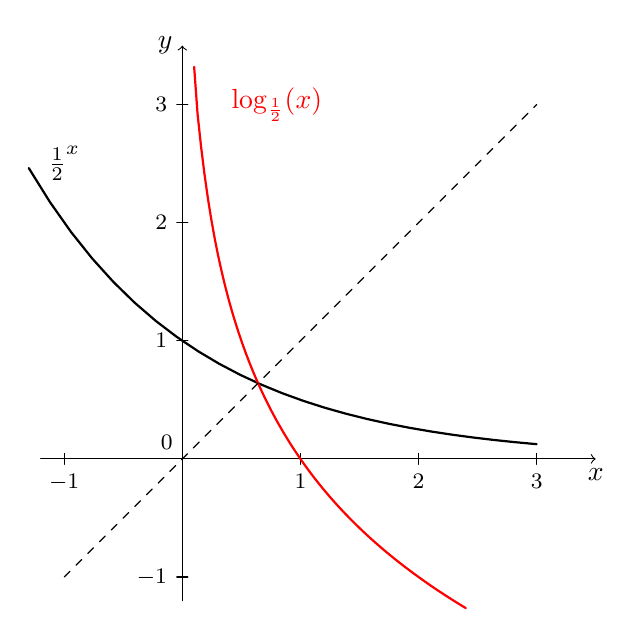
\begin{tikzpicture}[line cap=round,line join=round,x=1.5cm,y=1.5cm]
\draw[->] (-1.2,0) -- (3.5,0) node [at end, below] {$x$};
\foreach \x in {-1,1,2,3}
\draw[shift={(\x,0)}] (0pt,2pt) -- (0pt,-2pt) node[below] {\footnotesize $\x$};
\draw[->] (0,-1.2) -- (0,3.5) node [at end, left] {$y$};
\foreach \y in {-1,1,2,3}
\draw[shift={(0,\y)},color=black] (2pt,0pt) -- (-2pt,0pt) node[left] {\footnotesize $\y$};
\node[above left] (0,0) {\footnotesize $0$};
\draw [domain=-1.3:3,thick] plot(\x,{exp(\x*ln(0.5))});
\draw[] (-1,2.5) node {${\frac{1}{2}}^x$};
\draw [domain=0.1:2.4,samples=80,thick,red] plot(\x,{ln(\x)/ln(0.5)});
\draw[red] (0.8,3) node {$\log_{\frac{1}{2}}(x)$};
\draw[dashed] (-1,-1) -- (3,3);
\end{tikzpicture}
    \caption{Grafiek van $\log_{\frac{1}{2}}(x)$ en $(\frac12)^x$}
    \label{fig:log1/2}
\end{figure}
\begin{figure}[htb]
    \centering
        \begin{tikzpicture}[line cap=round,line join=round,x=1.5cm,y=1.5cm]
\draw[->] (-0.2,0) -- (4,0) node [at end, below] {$x$};
\foreach \x in {1,...,3}
\draw[shift={(\x,0)}] (0pt,2pt) -- (0pt,-2pt) node[below] {\footnotesize $\x$};
\draw[->] (0,-1.8) -- (0,2.8) node [at end, left] {$y$};
\foreach \y in {-1,1,2}
\draw[shift={(0,\y)},color=black] (2pt,0pt) -- (-2pt,0pt) node[left] {\footnotesize $\y$};
\node[below left] (0,0) {\footnotesize $0$};
\draw [domain=0.2:3.5,thick,blue,samples=80] plot(\x,{ln(\x)/ln(0.5))});
\draw[blue] (0.8,2) node {$\log_{\frac{1}{2}}(x)$};
\draw [domain=0.3:3.5,samples=80,thick,red] plot(\x,{ln(\x)/ln(2)});
\draw[red] (0.8,-1.8) node {$\log_{2}(x)$};
\end{tikzpicture}
    \caption{Grafiek van $\log_{\frac{1}{2}}(x)$ en $\log_2(x)$}
    \label{fig:loggroterkleiner}
\end{figure}
\begin{enumerate}
\setcounter{enumi}{4}
    \item  De logaritmische functie met grondtal $g$ kleiner dan 1 is \emph{dalend} op haar domein. 

    \item  Als $x$ nadert naar 0 dan worden de functiewaarden erg positief. Voor grote (positieve) waarden van $x$ wordt de functiewaarde erg negatief.
    \[
    \lim_{x\rightarrow0}\log_g(x)=+\infty \qquad \lim_{x\rightarrow+\infty}\log_g(x)=-\infty
    \]

\end{enumerate}


\subsection{Rekenregels}

De rekenregels voor machten zijn dezelfde als die voor de
exponenti\"{e}le functie. De logaritmische functie is \emph{de inverse functie} van de exponenti\"{e}le
functie. Er is dus een \emph{verband} tussen de
rekenregels van de logaritmische functie en die van de exponenti\"{e}le
functie, wat samengevat wordt in \cref{tbl:logexpverband}. 
\begin{table}[htbp]
    \centering
    \caption{Rekenregels voor exponenten en logaritmen}
       \begin{tabular}{p{5cm}|p{5.5cm}}
    \toprule
     & \emph{Als x en y positief zijn}  \\
    \midrule
    $g^{x+y}=g^{x}\cdot g^{y}$ & $\log_{g}(x\cdot y)=\log_{g}(x)+\log_{g}(y)$  \\  
    %\hline
    de `optelling van de argumenten' wordt omgezet naar `het product
    van functiewaarden' & de logaritme zet het
    `product van argumenten' om naar de  `som van
    functiewaarden'  \\     \midrule
    $g^{x\cdot y}=\left(g^{x}\right)^{y}=\left(g^{y}\right)^{x}$ & $\log_{g}(x^{y})=y\cdot \log_{g}(x)$
    \\  
    %\hline
    Het `product van argumenten' wordt omgezet naar een `macht
    van de functiewaarde' &
    De logaritme zet de ‘macht van de argumenten’ om naar `het
    product van de exponent met de functiewaarde'\\
    \midrule
   
    $g^{-x}=\frac{1}{g^{x}}$ & $\log_{g}\left(\frac{1}{x}\right)=-\log_{g}(x)$\\      %\hline
    het `tegengestelde van het argument' wordt omgezet naar het
    `omgekeerde van de functiewaarde' & de logaritme zet ‘omgekeerde
    van het argument’ om naar  het  `tegengestelde van de
    functiewaarde'  \\
    \bottomrule
\end{tabular}

    \label{tbl:logexpverband}
\end{table}

\newpage
\section{Exponenti\"{e}le vergelijkingen}
\label{sec:exp_vgl}
In wat volgt leren we vergelijkingen oplossen waar  de onbekende
in de exponent voorkomt. We spreken dan van een exponenti\"{e}le
vergelijking. 

Neem het voorbeeld van het kapitaal uit \cref{subsec:stijgendGroeiproces}. Je kan je afvragen na hoeveel jaar het kapitaal aangegroeid is tot \euros{1700}. Of   hoe lang het duurt totdat er in de ballon uit \cref{subsec.ballon} maar \SI{750}{\ml} draaggas overblijft. Om deze vragen op te lossen moet je een exponentiële vergelijking oplossen.

De algemene oplossingsmethode is als volgt:
\begin{enumerate}
\item Breng de factoren die de onbekende bevatten naar het linkerlid. De andere factoren breng je naar het rechterlid.
\item Schrijf het linkerlid als \'e\'en macht van de onbekende.
    \item  Pas de logaritmische functie toe op beide leden van de vergelijking. Gebruik 
    de eigenschappen en rekenregels (\cref{tbl:logexpverband}) van de logaritmische functie (zie hoger). 
    Zo bekom je een vergelijking waarbij de onbekende niet meer in de exponent voorkomt.
    \item Los die vergelijking op.
\end{enumerate}

\subsection{Voorbeeld 1}
Los volgende exponenti\"{e}le vergelijking op 
\begin{equation}
\left( \frac{1}{2}\right)^{x}=8
\label{exp_vgl:een}
\end{equation}


 \subsubsection{Analytische oplossing}
 De onbekende $x$ staat enkel in het linkerlid. Dit lid staat bovendien reeds als een macht van $x$. 
We kunnen dus starten bij de tweede stap van de algemene oplossingsmethode.
\begin{enumerate}
\addtocounter{enumi}{1}
\item Schrijf het linkerlid als \'e\'en macht van $x$.
\[
\left(\frac{1}{2}\right)^{x} =  8 
\]
\item Pas de logaritmische functie toe op beide leden van de gelijkheid.
\[
\log\left[ \left(\frac{1}{2}\right)^{x}\right] =  \log(8)
\]
\item Los de vergelijking op
\begin{align*}
     x\cdot \log\left(\frac{1}{2}\right) &=  \log(8)  \\
      &\Updownarrow  \\
     x &=  \frac{\log(8)}{\log\left(\frac{1}{2}\right)}  \\
      &\Updownarrow  \\
     x &= -3
 \end{align*}
\end{enumerate}
 Dit antwoord hadden we natuurlijk verwacht want deze vergelijking
 oplossen is zoeken naar \emph{de exponent, die we aan $\frac{1}{2}$
 moeten geven, om 8 te bekomen}.

 We kunnen vergelijking~\eqref{exp_vgl:een} ook omvormen tot beide leden
 geschreven zijn als een macht van hetzelfde grondtal, bvb.\ 2:
 \begin{displaymath}
     2^{-x}=2^{3}
 \end{displaymath}
Omdat  de exponenti\"ele functie een één-op-één relatie is (zie \cref{subsec.ggroter1}, nummertje~\ref{exp_func:inject}) vinden we snel
\begin{displaymath}
    -x=3 \Leftrightarrow x=-3
\end{displaymath}


\subsubsection{Grafische oplossing}
We kunnen vergelijking~\eqref{exp_vgl:een} ook beschouwen als het snijpunt van de functie $y=8$ met 
de exponenti\"{e}le functie
$y=\left(\frac{1}{2}\right)^{x}$. In \cref{fig:snijp1} zijn beide functies getekend. Je ziet dat $(-3,8)$ inderdaad het snijpunt is van beide functies. 
\begin{figure}[htbp]
    \centering
        \begin{tikzpicture}[line cap=round,line join=round,x=1cm,y=0.7cm]
\draw[->] (-3.2,0) -- (3.5,0) node [at end, below] {$x$};
\foreach \x in {-3,...,3}
\draw[shift={(\x,0)}] (0pt,2pt) -- (0pt,-2pt) node[below] {\footnotesize $\x$};
\draw[->] (0,-0.2) -- (0,9.5) node [at end, left] {$y$};
\foreach \y in {1,...,9}
\draw[shift={(0,\y)},color=black] (2pt,0pt) -- (-2pt,0pt) node[left] {\footnotesize $\y$};
\draw [domain=-3.2:3.2,thick,blue] plot(\x,{exp(\x*ln(0.5))});
\draw[blue] (-2.5,9) node {${\left(\dfrac{1}{2}\right)}^x$};
\draw[thick,red] (-3.5,8) -- (3,8) node[very near end,above] {$y=8$};
\draw [dashed, gray] (-3,0) -- (-3,8);
    \filldraw [gray] (-3,8) circle (2pt);
\end{tikzpicture}
    \caption{Snijpunt van de exponenti\"{e}le functie y=$(\frac12)^x$ en de rechte $y=8$}
    \label{fig:snijp1}
\end{figure}



\subsection{Voorbeeld 2}
In dit voorbeeld herwerken we het voorbeeld van het kapitaal uit \cref{subsec:stijgendGroeiproces} een weinig.
\begin{quote}

Een kapitaal van \euros{1000} staat uit tegen een
jaarlijkse rentevoet van \SI{7}{\percent}. Een ander kapitaal van \euros{2000} staat uit tegen een rentevoet van \SI{4}{\percent}. Wanneer zijn beide kapitalen evenveel waard?
\end{quote}


\subsubsection{Analytische oplossing}
Zij $K_1(t)$ de groeifunctie van het kapitaal dat uitstaat tegen \SI{7}{\percent} en $K_2(t)$ de groeifunctie van het kapitaal dat uitstaat tegen \SI{4}{\percent}. Analoog aan \cref{subsec:stijgendGroeiproces} leiden we de groeifuncties van beide kapitalen af:
\begin{equation}
\begin{split}
K_1(t)&=1000\cdot 1,07^t\\
K_2(t)&=2000\cdot 1,04^t
\end{split}
\end{equation}
We moeten $t$ zoeken zodat 
\begin{equation}
\begin{split}
K_1(t)&=K_2(t)   \\
&\Updownarrow\\
1\,000\cdot 1,07^t&=2\,000\cdot 1,04^t
\end{split}
\label{exp_vgl:vb2}
\end{equation} 
waarbij $t$ het aantal jaar weergeeft dat het geld op de bank staat.

We vereenvoudigen de vergelijking en passen de algemene
oplossingsmethode toe. 

\begin{enumerate}
\item Breng alle factoren die de onbekende $t$ bevatten naar het linkerlid.
\[
    \frac{\num{1.07}^t}{\num{1.04}^{t}}=\frac{2\,000}{1\,000}
\]
\item Schrijf het linkerlid als \'e\'en macht van $t$.
\[
\left(\frac{\num{1.07}}{\num{1.04}}\right)^{t}=\frac{2\,000}{1\,000}
\]
\item Pas de logaritmische functie toe op beide leden van de gelijkheid.
\begin{align*}
\log\left[\left(\frac{\num{1.07}}{\num{1.04}}\right)^{t}\right]&= \log\left(\frac{2\,000}{1\,000}\right)\\
     &\Updownarrow  \\
t\cdot \log\left(\frac{\num{1.07}}{\num{1.04}}\right)&= \log\left(\frac{2\,000}{1\,000}\right)
\end{align*}
\item Los de vergelijking op.
\[
t=\frac{\log\left(\dfrac{2\,000}{1\,000}\right)}{\log\left(\dfrac{\num{1.07}}{\num{1.04}}\right)}=\num{24.374033}
\]
\end{enumerate}

We vinden dat beide kapitalen ongeveer evenveel waard zijn na ruim 24 jaar.


Net zoals bij het eerste voorbeeld, kan de exponenti\"ele vergelijking~\eqref{exp_vgl:vb2} ook grafisch opgelost worden. In \cref{fig:snijp2} tekenen we de functies $f(x)=1\,000\cdot \num{1.07}^t$ en $g(x)=2\,000\cdot \num{1.04}^t$. We zien dat de functies mekaar snijden in $x=\num{24.37}$.
\begin{figure}[htbp]
    \centering
           \begin{tikzpicture}[line cap=round,line join=round,x=0.4cm,y=0.002cm]
\draw[->] (-0.2,0) -- (28,0) node [at end, below] {$x$ (jaar)};
\foreach \x in {0,2,...,26}
\draw[shift={(\x,0)}] (0pt,2pt) -- (0pt,-2pt) node[below] {\footnotesize $\x$};
\draw[->] (0,0) -- (0,5700) node [at end, left] {$y$ (\euro)};
\foreach \y in {500,1000,...,5500}
\draw[shift={(0,\y)},color=black] (2pt,0pt) -- (-2pt,0pt) node[left] {\footnotesize $\y$};
\draw [domain=-0:26,samples=50,thick,blue] plot(\x,{2000*exp(\x*ln(1.04))}); 
\draw[blue] (6,3000) node {$f(x)=\num{2000}\cdot \num{1,04}^x$};
\draw [domain=0:25.5,thick,red] plot(\x,{1000*exp(\x*ln(1.07))});
\draw[red] (10,1400) node {$g(x)=\num{1000}\cdot \num{1,07}^x$};
\draw[dashed,gray] (24.37,0) |- (0,5201);
    \filldraw [] (24.37,5202) circle (2pt) node[below right] { $(24,37;5202)$};
\end{tikzpicture}
    \caption{Snijpunt van de functies $f(x)=2000\cdot \num{1.04}^x$ \\en $g(x)=1000\cdot \num{1.07}^x$.}
    \label{fig:snijp2}
\end{figure}

\subsection[Stijgend groeiproces: verdubbelingstijd]{Voorbeeld 3: Verdubbelingstijd van een stijgend groeiproces}

  \begin{quote}
 Een bedrag van \euros{1000} staat op een spaarrekening met jaarlijkse intrest van \SI{7}{\percent}. Hoeveel jaar duurt het vooraleer het bedrag op de spaarrekening dubbel zo groot is?
\end{quote}
In \cref{subsubsec.si} vonden we het functievoorschrift dat de aangroei van het
kapitaal in de tijd weergeeft (vergelijking \eqref{eq:si}):
 \begin{displaymath}
     K(t)=1000\cdot \num{1.07}^{t}
 \end{displaymath}
Om het hierboven beschreven probleem op te lossen, moeten we de tijd $t$ vinden waarvoor het kapitaal $K(t)$ gelijk is  aan 2000:
\[
1000\cdot \num{1.07}^{t}  =  2000 
\]
\begin{enumerate}
\item Alle factoren waar $t$ in voorkomt naar het linkerlid brengen
\[
\num{1.07}^{t}=\frac{2000}{1000}=2
\]
\addtocounter{enumi}{1}
\item Logaritmische functie toepassen op beide leden van de gelijkheid
\[
\begin{split}
\log \left(\num{1.07}^{t} \right)&=\log 2\\
&\Updownarrow \\
t\log \left(\num{1.07} \right)&=\log 2
\end{split}
\]
\item Los de vergelijking op
\[
t=\frac{\log 2}{\log \left(\num{1.07} \right)}=\num{10.24}
\]
\end{enumerate}

Er stelt nu zich volgend probleem:
 \begin{quote}
 We hebben net berekend dat na $t=\num{10.24}$ jaar, te beginnen bij $t=0$,  het bedrag op de spaarrekening verdubbeld is.\emph{ Is het gekozen begintijdstip belangrijk?} M.a.w., verdubbelt het bedrag op de spaarrekening bijvoorbeeld ook in de periode van $t=4$ tot $t=\num{14.24}$?
 \end{quote}
 Om deze vraag te beantwoorden, berekenen we hoeveel tijd er nodig is om het bedrag op de spaarrekening te laten aangroeien van $1000$ tot $2\cdot K(4)$. We moeten dus $t$ zoeken zodat 
 \[
1000\cdot \num{1.07}^t= 2\cdot K(4)
 \]
 Omdat 
 \[
 K(4)=1000\cdot \num{1.07}^4
 \]
 geeft dit
 \[
 1000\cdot \num{1.07}^t=2\cdot 1000\cdot \num{1.07}^4
 \]
 We lossen deze vergelijking op.
 \begin{enumerate}
 \item $\displaystyle 
     \num{1.07}^{t} =  2 \cdot \num{1.07}^{4} $
 \addtocounter{enumi}{1}
 \item $\displaystyle 
     t\log(\num{1.07}) =  \log\left(2\cdot \num{1.07}^{4}\right) $
 \item $\displaystyle 
     t =  \frac{\log\left(2\cdot \num{1.07}^{4}\right)}{\log(\num{1.07})}=\num{14.24}$
 \end{enumerate}
 In de periode van $t=4$ tot $t=\num{14.24}$ verdubbelt het kapitaal op het spaarboekje dus ook. Ongeacht het begintijdstip, duurt het altijd \num{10.24} jaar voordat het kapitaal verdubbelt.
 
 Op analoge manier kan je berekenen dat \emph{het beginkapitaal geen invloed heeft op de tijd die nodig is om het beginkapitaal te verdubbelen.} Met andere woorden: de benodigde tijd hangt enkel af van de groeifactor $g=\num{1.07}$.
 
 \subsubsection{Definitie}
 \begin{quote}
 De verdubbelingstijd\index{verdubbelingstijd} $t_v$ is de tijd die bij een stijgend exponentieel groeiproces $B(t)=B(0)\cdot g^t$ nodig is  om  de functiewaarde van $B(t)$ te verdubbelen.  De verdubbelingstijd is enkel afhankelijk van de groeifactor $g$ en is gelijk aan 
 \begin{displaymath}
     t_{v}=\frac{\log(2)}{\log(g)}
 \end{displaymath} 
 \end{quote}
 De verdubbelingstijd is \emph{onafhankelijk}
 van de beginwaarde $B(0)$ of het tijdstip waarop men die berekent. 



 \subsection[Dalend groeiproces: halveringstijd] {Voorbeeld 4: Halveringstijd van een dalend groeiproces}

 Wanneer we te maken hebben met een dalend groeiproces is het zinloos
 te vragen naar de verdubbelingstijd, maar kunnen we enkel \emph{de
  halveringstijd} zoeken.  We hernemen het voorbeeld van \cref{subsec.ballon}.
  \begin{quote}
  Een luchtballon verliest  \SI{5}{\percent} van zijn
 draaggas per dag. Oorspronkelijk is er \SI{1000}{\milli\litre} gas aanwezig.
     Na hoeveel dagen zal de hoeveelheid draaggas in de ballon gehalveerd zijn?
 \end{quote}
We zoeken dus tijdstip $t$ waarvoor de hoeveelheid draaggas $D(t)=500$. We maken gebruik van vergelijking \eqref{eq:ballon}:
\[
     1000\cdot \num{0.95}^{t} =  500  
     \]
     \begin{enumerate}
\item $\displaystyle      
     \num{0.95}^{t} =\frac{1}{2}$
     \addtocounter{enumi}{1}
\item $\displaystyle      
     \log(\num{0.95}^{t}) =  \log\left(\frac{1}{2}\right) $
\item $\displaystyle      
     t =  \frac{\log(\frac{1}{2})}{\log(\num{0.95})} \label{eq:th_draaggas}
$
     \end{enumerate}
     Het duurt dus  \num{13.51} dagen voordat de hoeveelheid draaggas gehalveerd is. We merken op dat in bovenstaande  vergelijking enkel de groeifactor $g=\num{0.95}$ voorkomt en niet de beginwaarde 1000 of het begintijdstip $t=0$.

 \subsubsection{Definitie}
 \begin{quote}
 De halveringstijd\index{halveringstijd} $t_h$ is de tijd die bij een dalend exponentieel groeiproces $B(t)=B(0)\cdot g^t$ nodig is  om  de functiewaarde van $B(t)$ te halveren.
 De halveringstijd is enkel afhankelijk van de groeifactor $g$ en is gelijk aan 
 \begin{displaymath}
     t_{h}=\frac{\log(\frac{1}{2})}{\log(g)}
 \end{displaymath} 
 \end{quote}


\subsection{Voorbeeld 5}

Los volgende vergelijking op:
\begin{equation}
    4^{x}+7\cdot 2^{x}-8=0
\label{eq:vb3}
\end{equation}
We brengen de termen die de veranderlijke $x$ bevatten naar het linkerlid:
\begin{equation*}
4^x+7\cdot 2^x=8
\end{equation*}
Omwille van de som in het linkerlid van vergelijking~\eqref{eq:vb3} kunnen we dit niet schrijven als \'e\'en macht van $x$. We kunnen de tweede stap van de algemene oplossingsmethode dus niet uitvoeren. In de derde stap moeten we de logaritme van beide leden nemen. We merken dat we de veranderlijke $x$ niet uit de logaritme kunnen isoleren omwille van de som. We hebben dus een andere oplossingsmethode nodig, namelijk substitutie. Bij substitutie vervangen we een `stuk' van de vergelijking door een nieuwe veranderlijke in de hoop dat de vergelijking wel opgelost kan worden naar die nieuwe veranderlijke. 

In dit geval stellen we als substitutie $z=2^x$ voor.
Dit is de eenvoudigste
macht van 2 die in de vergelijking voorkomt.
We schrijven alle termen in de vergelijking in functie van $z$
zodat $x$ uit de vergelijking verdwijnt:
\begin{align*}
    \left(2^{2}\right)^{x}+7\cdot2^{x}-8 &= 0  \\
     &\Updownarrow  \\
    \left(2^{x}\right)^{2}+7\cdot2^{x}-8 &=  0  \\
     &\Updownarrow \text{ stel } z=2^x \\
    z^{2}+7\cdot z-8 &= 0
\end{align*}
Deze tweede graadsvergelijking heeft als oplossingen $z=1$ en $z=-8$.
We vervangen $z$ opnieuw door $2^{x}$. 

Als $z=1$ bekomen we de eenvoudige exponenti\"ele vergelijking
\[
 2^{x}  =  1
\]
Deze vergelijking kunnen we oplossen met de algemene oplossingsmethode:
\begin{align*}
    \log\left(2^x\right) &=  \log(1) \\
     &\Updownarrow  \\
    x\cdot \log(2) &= 0 \\
     &\Updownarrow  \\
    x &=  0
\end{align*}

Als $z=-8$ bekomen we na de substitutie
 \begin{displaymath}
    2^{x} = -8  
    \end{displaymath}
    Deze  vergelijking is \emph{niet oplosbaar} want een macht van 2 is steeds positief en kan dus nooit gelijk zijn aan $-8$. 
    
   De enige oplossing voor vergelijking~\eqref{eq:vb3} is bijgevolg $x=0$.

    \subsection{Voorbeeld 6}
    Een schijnbaar eenvoudige vergelijking als
    \begin{displaymath}
        2^{x}+x = 0
    \end{displaymath}
      kan niet exact opgelost worden. Deze
      vergelijking kan \emph{enkel numeriek of grafisch} opgelost worden.
      Bij een numerieke oplossing zoekt de computer via een (gekend) algoritme\footnote{Enkele gekende algoritmen zijn `Regula Falsi' (\url{http://nl.wikipedia.org/wiki/Regula\_falsi}) en de `methode van Newton Raphson' (\url{http://nl.wikipedia.org/wiki/Newton-Raphson}).} een benaderende oplossing van de vergelijking. 
      Bij de grafische oplossing zoeken we op een grafiek het snijpunt van de functies $f(x)=2^x$ en $g(x)=-x$.
      Op \cref{fig:snijp3} lees je af dat de oplossing ongeveer $x=\num{-0.64}$ is.
\begin{figure}[htbp]
  \centering
  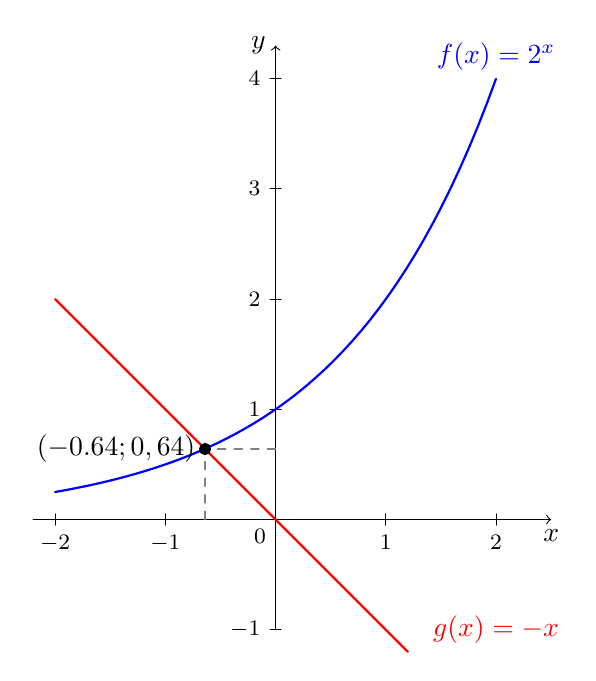
\begin{tikzpicture}[line cap=round,line join=round,x=1.4cm,y=1.4cm]
    \draw[->] (-2.2,0) -- (2.5,0) node [at end, below] {$x$};
    \foreach \x in {-2,-1,1,2}
    \draw[shift={(\x,0)}] (0pt,2pt) -- (0pt,-2pt) node[below] {\footnotesize $\x$};
    \draw[->] (0,-1) -- (0,4.3) node [at end, left] {$y$};
    \foreach \y in {-1,1,,2,...,4}
    \draw[shift={(0,\y)},color=black] (2pt,0pt) -- (-2pt,0pt) node[left] {\footnotesize $\y$};
    \node[below left] (0,0) {\footnotesize $0$};
    \draw [domain=-2:2,samples=50,thick,blue] plot(\x,{exp(\x*ln(2))}); 
    \draw[blue] (2,4.2) node {$f(x)=\num{2}^x$};
    \draw [thick,red] (-2,2) -- (1.2,-1.2) ;
    \draw[red] (2,-1) node {$g(x)=-x$};
    \draw[dashed,gray] (-0.64,0) |- (0,0.64);
    \filldraw [] (-0.64,0.64) circle (2pt) node[left] { $(\num{-0.64};\num{0,64})$};
  \end{tikzpicture}
  \caption{Snijpunt van de functies $f(x)=2^x$ en $g(x)=-x$}
  \label{fig:snijp3}
\end{figure}


% Sectie "Logaritmische vergelijkingen" staat in oud/logvgl.tex

\section{Samenvatting}
\paragraph{Exponenti\"ele functies}
\[
  f(x) = g^x
\]
\paragraph{Rekenregels exponenti\"ele functies}
\[
  \begin{array}{rclcl}
    g^{x+y}  & = & g^x \cdot g^y                     \\ \\
    \displaystyle (g^x)^y & = & \displaystyle (g^y)^x           & = & g^{x \cdot y} \\ \\
    \displaystyle g^{-x}   & = & \displaystyle \frac{1}{g^x}
  \end{array}
\]
\paragraph{Logaritmische functies}
\[
  y = \log_g(x) \iff g_y = x
\]
\paragraph{Rekenregels logaritmische functies}
\[
  \begin{array}{rcl}
    \log_g(x \cdot y) & = & \log_g x + \log_g y \\ \\
    \log_g(x^y) & = & y \cdot \log_g x \\ \\
    \displaystyle \log_g(\frac1x) & = & -\log_g x
  \end{array}
\]


%%%%%%%%%%%%%%%%%%%%%%%%%%%%%%%%%
% Laatste aanpassing:           %
% 6 sept 2013 [Jan]: kleine aanpassingen
% 28/06/13 [Greetje]: Verbeterd en examenvragen van Leentje toegevoegd
% 23/3/11 [Greetje]: Volledig herwerkt
%
% 10/09/01 door Greetje
%   verbeteringen van Roos
%   rekenregels weggelaten
%
% 01/09/01 door Greetje          %
%%%%%%%%%%%%%%%%%%%%%%%%%%%%%%%%%

\section{Oefeningen}
\begin{oef}     
Los de volgende vergelijkingen op naar $x$. 
\begin{multicols}{2}
\begin{enumerate}
  \item $3^{-x+2}=0,7^{2\cdot x}$
  \item $4^{x}-5\cdot 2^{x}-24=0$
  \item $3^{x}+3^{x+1}=4$
  \item $3^{x+1}-26=3\cdot 3^{-x}$
  \item $2^{3^x}=8$
  \item $9^{x+1}-2\cdot 3^{x+2}-27=0$
  \item $5^{x+1}=5^{3x+1}$
  \item $2^{x+3}=16^{x-3}$
  \item $3^x=59049$
  \item $\left(\frac12\right)^x=2048$
  \item $7^x=2\cdot 8^x$
  \item $2^{x+3}=16^{x-3}$
  \item $100 \cdot 1,05^x=2000\cdot 1,025^x$
  \item $15\cdot 3^{x+1}-243\cdot 5^{x-2}=0$
  \item $3^{4x+5}=5^{x-1}$
  \item $512 + 2^{2x} = 2^{4+x}+2^{5+x}$
\end{enumerate}
\end{multicols}
\begin{opl}
\begin{enumerate}
  \item \[
          \begin{array}{rrclcl}
                 & 3^{-x+2} & = & 0.7^{2x} \\
            \iff & 9 \cdot 3^-x & = & 0.7^{2x} \\
            \iff & 9 & = & 0.7^{2x} \cdot 3^x \\
            \iff & 9 & = & (0.7^2 \cdot 3)^x \\
            \iff & \log(9) & = & x \log(0.7^2 \cdot 3) \\
            \iff & x & = & \frac{\log(9)}{\log(0.7^2 \cdot 3)} & \approx & 5.70319
          \end{array}
        \]
  \item \[
          \begin{array}{rrclcl}
                 & 4^x - 5 \cdot 2^x - 24 = 0
            \iff & (2^x)^2 - 5 \cdot 2^x - 24 = 0
          \end{array}
        \]
        We voeren $z = 2^x$ in, dit geeft ons
        \[
          z^2 - 5z - 24 = 0
        \]
        Dit is een vierkantsvergelijking met als discriminant
        \[
          D = (-5)^2 - 4 \cdot 1 \cdot (-24) = 25 + 4 \cdot 24 = 121
        \]
        en met twee oplossingen
        \[
          z_1 = \frac{5 - \sqrt{D}}{2} = -3 \qquad z_2 = \frac{5+\sqrt{D}}{2} = 8
        \]
        Dit geeft ons
        \[
          2^{x_1} = -3 \qquad 2^{x_2} = 8
        \]
        De linkervergelijking heeft geen oplossing, de rechter heeft als oplossing $x_2 = \log_2(8) = 3$.
  \item \[
          \begin{array}{rrclcl}
                 & 3^x+3^{x+1} & = & 4 \\
            \iff & 3^x+3^x\cdot3 & = & 4 \\
            \iff & 3^x(1+3) & = & 4 \\
            \iff & 3^x & = & 1 \\
            \iff & x & = & 0
          \end{array}
        \]
  \item \[
          \begin{array}{rrclcl}
                 & 3^{x+1}-26 & = & 3 \cdot 3^{-x} \\
            \iff & 3^{2x+1}-26 \cdot 3^x & = & 3 \\
            \iff & 3 \cdot (3^x)^2-26 \cdot 3^x - 3 & = & 0 \\
          \end{array}
        \]
        Substitutie $z = 3^x$
        \[
          3 z^2 - 26 z - 3 = 0
        \]
        Dit is een vierkantsvergelijking met
        \[
          D = (-26)^2 - 4 \cdot 3 \cdot (-3) = 712
        \]
        en
        \[
          z_1 = \frac{26 - \sqrt{D}}{6} \approx -0.11 \qquad z_2 = \frac{26 + \sqrt{D}}{6} \approx 8.78
        \]
        $z_1 = 3^x$ geeft ons geen oplossingen, maar
        \[
          \frac{26 + \sqrt{D}}{6} = 3^x \iff x = \log_3\left( \frac{26 + \sqrt{712}}{6} \right) \approx 1.98
        \]
  \item \[
          \begin{array}{rrclcl}
                 & 2^{(3^x)} & = & 8 \\
            \iff & 2^{(3^x)} & = & 2^3 \\
            \iff & 3^x & = & 3 \\
            \iff & x & = & 1
          \end{array}
        \]
  \item \[
          \begin{array}{rrclcl}
                 & 9^{x+1}-2 \cdot 3^{x+2}-27 & = & 0 \\
            \iff & 9 \cdot (3^x)^2 - 18 \cdot 3^x - 27 & = & 0
          \end{array}
        \]
        Substitutie $z = 3^x$
        \[
          9 z^2 - 18 z - 27 = 0
        \]
        Dit geeft een vierkantsvergelijking met
        \[
          D = (-18)^2 - 4 \cdot 9 \cdot (-27) = 1296 \qquad \sqrt{D} = 36
        \]
        en oplossingen
        \[
          z_1 = \frac{18 - 36}{18} = -1 \qquad z_2 = \frac{18 + 36}{18} = 3
        \]
        $z_1 = -1$ geeft geen oplossingen voor $x$, maar
        \[
          3 = 3^x \iff x = 1
        \]
  \item \[
          \begin{array}{rrclcl}
                 & 5^{x+1} & = & 5^{3x+1} \\
            \iff & 5^x & = & 5^{3x} \\
            \iff & x & = & 3x \\
            \iff & x & = & 0
          \end{array}
        \]
  \item \[
          \begin{array}{rrclcl}
                 & 2^{x+3} & = & 16^{x-3} \\
            \iff & 2^x \cdot 2^3 & = & 2^{3x} \cdot 2^{-9} \\
            \iff & 2^{10} & = & 2^{2x} \\
            \iff & 10 & = & 2x \\
            \iff & x & = & 5
          \end{array}
        \]
  \item $3^x=59049 \iff x = \log_3(59049) = 10$
  \item \[
          \begin{array}{rrclcl}
                 & \displaystyle \left(\frac12\right)^x & = & 2048 \\[2mm]
            \iff & 2^{-x} & = & 2^{11} \\
            \iff & x & = & -11
          \end{array}
        \]
  \item \[
          \begin{array}{rrclcl}
                 & 7^x & = & 2 \cdot 8^x \\[2mm]
            \iff & \displaystyle\left(\frac78\right)^x & = & 2 \\[2mm]
            \iff & \displaystyle x \cdot \log(\frac78) & = & \log(2) \\[2mm]
            \iff & x & = & \displaystyle \frac{\log(2)}{\log(7) - 3 \log(2)}
          \end{array}
        \]
  \item \[
          \begin{array}{rrclcl}
                 & 2^{x+3} & = & 16^{x-3} \\
            \iff & 2^x \cdot 2^3 & = & 2^{4x} \cdot 2^{-12} \\
            \iff & 2^{15} & = & 2^{3x} \\
            \iff & x & = & 5
          \end{array}
        \]
  \item \[
          \begin{array}{rrclcl}
                 & 100 \cdot 1,05^x & = & 2000\cdot 1,025^x \\[2mm]
            \iff & \displaystyle\left(\frac{1.05}{1.025}\right)^x & = & 20 \\[2mm]
            \iff & x & = & \displaystyle \frac{\log(20)}{\log(1.05)-\log(1.025)} & \approx & 124.3
          \end{array}
        \]
  \item \[
          \begin{array}{rrclcl}
                 & 15 \cdot 3^{x+1}-243 \cdot 5^{x-2} & = & 0 \\ 
            \iff & 15 \cdot 3^x \cdot 3 & = & 243 \cdot 5^x \cdot 25^{-1} \\[2mm]
            \iff & 3^x \cdot 5^{-x} & = & \displaystyle \frac{243}{15 \cdot 3 \cdot 25} \\[2mm]
            \iff & \displaystyle \left(\frac{3}{5}\right)^x & = & \displaystyle \frac{27}{125} \\[2mm]
            \iff & \displaystyle x \cdot \log\left(\frac{3}{5}\right) & = & \displaystyle \log\left(\frac{27}{125}\right) \\[2mm]
            \iff & \displaystyle x \cdot \log\left(\frac{3}{5}\right) & = & \displaystyle \log\left(\frac{3^3}{5^3}\right) \\[2mm]
            \iff & \displaystyle x \cdot \log\left(\frac{3}{5}\right) & = & \displaystyle 3 \cdot \log\left(\frac{3}{5}\right) \\[2mm]
            \iff & x & = & 3 
          \end{array}
        \]
  \item \[
          \begin{array}{rrclcl}
                 & 3^{4x+5} & = & 5^{x-1} \\
            \iff & 3^{4x} \cdot 3^5 & = & 5^{x} \cdot 5^{-1} \\[2mm]
            \iff & \left(3^4 \cdot 5^{-1}\right)^x & = & 5^{-1} \cdot 3^{-5} \\[2mm]
            \iff & x \cdot \log\left(3^4 \cdot 5^{-1}\right) & = & \log(5^{-1} \cdot 3^{-5}) \\[2mm]
            \iff & x & = & \displaystyle \frac{\log(5^{-1} \cdot 3^{-5})}{\log\left(3^4 \cdot 5^{-1}\right)} \\[3mm]
            \iff & x & = & \displaystyle \frac{-\log(5) - 5 \log(3)}{4\log(3) - \log(5)} & \approx & -2.55
          \end{array}
        \]
  \item \[
          \begin{array}{rrclcl}
                 & 512 + 2^{2x} & = & 2^{4+x}+2^{5+x} \\
            \iff & 2^9 + (2^x)^2 & = & (2^4 + 2^5) \cdot 2^x \\
            \iff & (2^x)^2 - (2^4 + 2^5) \cdot 2^x + 2^9 & = & 0 \\
            \iff & (2^x)^2 - 48 \cdot 2^x + 512 & = & 0
          \end{array}
        \]
        Substitutie $z = 2^x$.
        \[
          z^2 - 48 z + 512 = 0
        \]
        Dit is een vierkantsvergelijking met
        \[
          D = 48^2 - 4 \cdot 1 \cdot 512 = 256 \qquad \sqrt{D} = 16
        \]
        en oplossingen
        \[
          z_1 = \frac{48 - 16}{2} = 16 \qquad z_2 = \frac{48+16}{2} = 32
        \]
        Dit geeft voor $x$
        \[
          2^{x_1} = 16 \iff x_1 = 4 \qquad 2^{x_2} = 32 \iff x_2 = 5
        \]
\end{enumerate}
\end{opl}
\end{oef}

% Oefeningen op logaritmische vergelijkingen
%\begin{oef} $\qquad$
% \\
%\begin{multicols}{2}
%\begin{enumerate}
%\item   $3 \cdot \log_{2}2 +\log_{2}x=3$ 
%\\ \item   $\log_{x}(\sqrt{3})=3$
%\\ \item    $\log(2x+3)+\log(x-1)=\log(x^{2}+9)$
%\\ \item     $\log_{64}(\log_{x}(16))^{3}=1$ 
%\\ \item $(\log_{2}x)^{3}+\log_{2}(x^{4})=4\cdot (\log_{2}x)^{2}$
%\\ \item  $\displaystyle{\log_{2}x=\frac{1}{\log_{6-x}4}}$
%\\ \item $\log_{2}(2^{x}-7)+x=3$
%\\ \item $\log_{x}(2\cdot x+8)=2$ 
%\\ \item $\log(x-3)+\log(x+1)=\log(2x+2)$
%\\ \item  $\left[\log(x+2)\right]^3+\left[\log(x+2)\right]^2=\log\left[(x+2)^2\right]$
% \end{enumerate}
%    
%\end{multicols}
%
%     \end{oef}
     
\begin{oef}
Een blad papier is 1 mm dik. We plooien dit blad een
\emph{aantal keren na elkaar} dubbel. In de veronderstelling dat
we dit proces heel dikwijls na elkaar \emph{kunnen} uitvoeren,
hoeveel keren moeten we minstens plooien opdat de dikte van
het geplooide blad papier meer dan 2 cm zou meten?
\begin{opl}
Dikte van geplooide papier: $D(t)=2^t$.\\
Zoek $t$ zodat $D(t)=20$. Dit geeft $t=\log20/\log 2=4,32$.\\
Antwoord: na vijf keer plooien is dikte meer dan 2 cm.
\end{opl}
\end{oef}

\begin{oef}
We nemen aan dat op korte termijn de waarde van een aandeel stijgt
volgens een exponentieel  proces. Op 10 maanden is de prijs van
het aandeel verdrievoudigd.
\begin{enumerate}
  \item Bepaal de groeifactor (i) per 10 maand en (ii) per maand van dit groeiproces.
  \item Als je weet dat het aandeel nu het vijfvoud is van
        toen het werd aangekocht, hoeveel maanden geleden is het dan
        aangekocht?
\end{enumerate}
\begin{opl}
  \begin{enumerate}
    \item $g_{10}=3$; $g_m=3^\frac{1}{10}$
    \item Waarde van aandeel in functie van de tijd: $B(t)=B(0)\cdot 3^\frac{t}{10}$ \\
          Zoek $t$ zodat $B(t)=5B(0)$. Dat geeft $t=\log5/\log3^\frac{1}{10}=14,65$, dus na 14,65 maanden.
  \end{enumerate}
\end{opl}
\end{oef}

 
\begin{figure}[hbtp]
  \flushright
  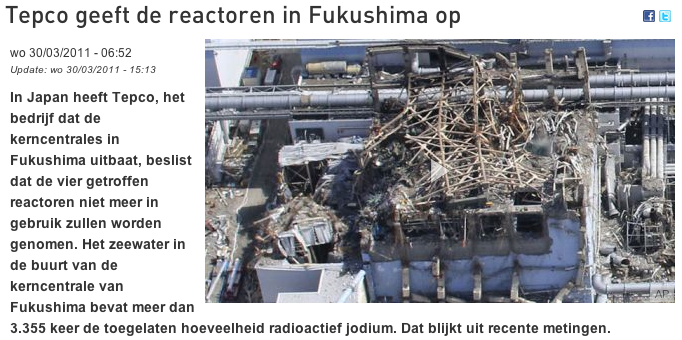
\includegraphics[width=0.95\textwidth]{oefeningen/jodiumderedactie.png}
  \caption{Fukushima -- De redactie, 30 maart 2011}
  \label{fig:fukushima} 
\end{figure}    

\begin{oef}
In 2011 werd Japan getroffen door een zware aardbeving met bijbehorende tsunami. De kernreactoren in Fukushima konden niet meer gekoeld worden en ontploften gedeeltelijk. Op 30 maart 2011 (figuur~\ref{fig:fukushima}) bleek de hoeveelheid radioactief Jodium in het zeewater ($\text{I}^{131}$) 3355 keer de toegelaten hoeveelheid te bedragen. 
De Japanse overheid beweerde dat er geen probleem was voor de consumptie van vis uit de zee, want de radioactiviteit zou snel verdund worden. Bereken hoelang het duurt (bij deze verontreiniging) tot de radioactiviteit van het $\text{I}^{131}$ terug gelijk is aan de toegelaten hoeveelheid. De halveringstijd van $\text{I}^{131}$ is 8 dagen.
\begin{opl}
\[
  J(t)=3355\cdot J_0\cdot \left( \frac12\right)^\frac{t}{8}
\]
Zoek $t$ zodat $J(t)=J_0$
\[
  t=8\frac{\log \frac{1}{3355}}{\log\frac12}\approx93,70
\]
dus na 93,70 dagen.
\end{opl}
\end{oef}


\begin{oef}
Op een archeologische site werden muurschilderingen
teruggevonden. De ouderdom van de schildering wordt bepaald
met de $\text{C}^{14}$-proef.  Men weet immers  dat de
hoeveelheid van dit isotoop jaarlijks exponentieel daalt met factor
\num{0.99988}. Op de schilderingen werd \SI{20}{\percent} van de
oorspronkelijke hoeveelheid $\text{C}^{14}$ teruggevonden. Hoe oud
zijn de schilderingen?
\begin{opl}
\[ C(t)=0,20\cdot C_0\cdot 0,9988^t \]
Zoek $t$ zodat $C(t)=C_0$\\
\[ t=\frac{\log5}{\log0,9988}\approx-13411\]
dus 13411 jaar geleden.
\end{opl}
\end{oef}

\begin{oef}
Jan zet \euros{1900} op een spaarboekje tegen samengestelde
intrest van \SI{5}{\percent} per jaar en \euros{1000} op een andere rekening,
waarvan de verdubbelingstijd van het kapitaal 25 jaar bedraagt.
Wanneer zal het bedrag op het spaarboekje dubbel zo
groot zijn als het bedrag op de rekening?
\begin{opl}
Groeifunctie van spaarboekje 1: $S_1(t)=1900\cdot 1,05^t$; \\Groeifunctie van spaarboekje 2: $S_2(t)=1000\cdot 2^\frac{t}{25}$\\
Zoek $t$ zodat $S_1(t)=2\cdot S_2(t)$, wat geeft $t=\frac{\log(19/20)}{\log(2^{1/25}/1,05)}=2,435$.\\
Antwoord: na 2,435 jaar is het bedrag van het spaarboekje dubbel zo groot als het bedrag op de rekening.
\end{opl}
\end{oef}

\begin{oef}
De waarde van een schilderij van Rembrandt neemt per
decennium (periode van 10 jaar) toe met \SI{20}{\percent}. De waarde van een schilderij
van Picasso stijgt in waarde met \SI{5}{\percent} per jaar. Een
kunsthandelaar koopt vandaag een schilderij van Rembrandt voor~\euros{300\,000}
en een schilderij van Picasso voor~\euros{225\,000}.
Wanneer zullen beide schilderijen evenveel waard zijn?
\begin{opl}
De waarde van de Rembrandt: $R(t)=300000\cdot 1,20^{t/10}$\\
De waarde van de Picasso: $P(t)=225000\cdot 1,05^t$\\
Zoek $t$ zodat $P(t)=R(t)$, wat geeft $t=\log(300/225)/\log(1,05/1,20^{1/10})=9,41$.\\
Antwoord: na 9,41 jaar zijn beide schilderijen evenveel waard.
\end{opl}
\end{oef}

\begin{oef}
Land A heeft 80 miljoen inwoners en land B heeft er 100
miljoen. De bevolking van land A verdubbelt in 20 jaar en die
van land B groeit elk jaar aan met \SI{2,3}{\percent}.
\begin{enumerate}
  \item Bereken de groeifactor per jaar van land A.
  \item Bereken de verdubbelingstijd voor land B.
  \item Wanneer zal het aantal inwoners van land A gelijk zijn
        aan dat van land B?
\end{enumerate}
\begin{opl}
$A(t)=80\cdot 2^{t/20}$; $B(t)=100\cdot 1,023^t$;\\
Zoek $t$ zodat $A(t)=B(t)$, wat geeft $t=\log(8/10)/\log(1,023/2^{1/20})=18,72$\\
Antwoord: na 18,72 jaar zal het aantal inwoners gelijk zijn.
\end{opl}
\end{oef}

\begin{oef}
Wim is nu 7 jaar oud en wil op zijn twaalfde
verjaardag een
fiets met 10 versnellingen als geschenk. Zijn ouders willen nu
reeds een bedrag op een spaarrekening zetten van \euros{400} tegen een
jaarlijkse rente van \SI{7}{\percent}.
\begin{enumerate}
  \item Over welk bedrag beschikt Wim op zijn twaalfde verjaardag?
  \item Wanneer zal het bedrag op Wim's spaarrekening verdubbeld zijn?
\end{enumerate}
\begin{opl}
  Groeifunctie die het gespaarde bedrag $t$ jaar na de zevende verjaardag weergeeft: $B(t)=400\cdot 1,07^t$\\
  \begin{enumerate}
    \item bedrag op rekening bij twaalfde verjaardag: $B(5)=561,02$
    \item Zoek $t$ zodat $B(t)=800$, wat geeft $t=\log2/\log1,07=10,24$, dus als Wim 17,24 jaar is, heeft hij 800\euros op zijn rekening staan.
  \end{enumerate}
\end{opl}
\end{oef}

\begin{oef}
Een vader wil nu een bedrag van \euros{10\,000} verdelen over zijn
2 kinderen van respectievelijk 10 en \num{14,5} jaar oud. De vader wil
dat de verdeling zo verloopt, dat elk kind later op zijn
\'{e}\'{e}nentwintigste verjaardag \emph{hetzelfde} kapitaal ontvangt.
De jaarlijkse rente op beide rekeningen is dezelfde en bedraagt \SI{7}{\percent}.
\begin{enumerate}
  \item Welk bedrag wordt nu voor elk kind belegd?
  \item Over welk bedrag zal ieder kind beschikken op zijn
        \'e\'enentwintigste verjaardag?
\end{enumerate}
\begin{opl}
Bedrag op rekening van kind 1: $B_1(t)=B_1\cdot 1,07^t$ met $t$ het aantal jaren sinds `nu'.\\
Bedrag op rekening van kind 2: $B_2(t)=B_2\cdot 1,07^t$ met $B_1+B_2=\num{10000}$; \\
Zoek $B_1$ en $B_2$ zodat $B_1(11)=B_2(6,5)$. Omdat $B_1+B_2=\num{10000}$, moeten we $B_1$ zoeken zodat 
$B_1\cdot 1,07^{11}=(10000-B_1)\cdot 1,07^{6,5}$, wat geeft $B_1=4244$. \\
Antwoord: Nu wordt \euros{4244} en \euros{5755} belegd.\\
Op zijn  \'{e}\'{e}nentwintigste verjaardag zal het kind beschikken over \euros{8934}.
\end{opl}
\end{oef}

\begin{oef}
Een kapitaal van \euros{3000} wordt uitgezet tegen samengestelde intrest
en groeit aan tot \euros{\num{4432.37}} na 8 jaar. Na hoeveel tijd is dit bedrag \euros{5000} geworden?
\begin{opl}
Eerst zoeken we de groeifactor uit de vergelijking:\\
$3000\cdot g^{8} = 4432,37$\\
Hieruit vinden we dat $g$ gelijk is aan $1,05$. Het kapitaal groeit dus met \SI{5}{\percent} per jaar.\\
Nu kunnen we berekenen wanneer het kapitaal aangegroeid is tot \euros{5000}\\
$3000\cdot 1,05^{t} = 5000$\\
$t = \log(5/3)/\log(1,05)$\\
$t = 10,46$\\
Hieruit vinden we dat het kapitaal $11$ jaar op de bank moet blijven staan vooraleer het is aangegroeid tot \euros{5000}.
\end{opl}
\end{oef}
  

% Opm. Inge: oefening is wat verwarrend, doders doen in het begin niets? Vreemd. Beter weglaten   
%\begin{oef}
%   Het is nat en koud en je hebt een stevige bronchitis te pakken. De dokter laat bloed nemen en stelt vast dat je \SI{40500} bacteriën in je bloed hebt, die zich ieder etmaal (=\SI{24}{\hour)} verdubbelen in aantal. Je zit midden in de examenperiode en wilt zo snel mogelijk van die kleine ettertjes verlost worden. De dokter injecteert je met een hoge concentratie bacterie-doders. Na de injectie heb je 3000 bacterie-doders in je bloed, die zich iedere \SI{8}{\hour} verdubbelen. Je zult je stukken beter voelen zodra het aantal bacterie-doders groter wordt dan het aantal bacteriën. Na hoeveel uur zal je van je bronchitis verlost zijn? 
%   \begin{enumerate}
%\item Bereken zowel  voor de kolonie bacteriën als voor de bacterie-doders de groeifactor per uur.
%
%\item Stel de vergelijkingen op die hun groei simuleren.
%
%\item Reken uit na hoeveel uur hun aantallen gelijk worden en je de strijdt tegen je bronchitis wint.
%
%   \end{enumerate}
%   \begin{opl}
%   $B(t)=40500\cdot 2^{t/24}$; $D(t)=3000\cdot 2^{t/8}$. Na \SI{5,2} uur zijn er meer bacterie-doders dan bacteriën.
%   \end{opl}
%   \end{oef}

\begin{oef}
Het wordt steeds duidelijker dat de mensen wegtrekken uit de grote steden in Belgi\"e.
Brussel had in 2010 nog \num{1124000} inwoners, en ziet zijn inwonertal dalen met \SI{10}{\percent}
per decennium (= 10 jaar). Leuven en omstreken blijken echter zeer gegeerd. Met een
inwonertal van \num{95500} in 2010 was Groot-Leuven nog een kleine stad. Het lijkt
er echter op dat dit inwonertal zal verdubbelen per 8 jaar. Hoe lang duurt het
vooraleer Leuven en Brussel even groot geworden zijn?
\begin{enumerate}
  \item Bereken voor het aantal inwoners van Brussel en Leuven de jaarlijkse groeifactor.
  \item Stel de vergelijkingen op die de groei/daling van de bevolking in Brussel en Leuven simuleren.
  \item Reken uit na hoeveel jaar Leuven evenveel inwoners telt als Brussel.
\end{enumerate}
\begin{opl}
$B(t)=\num{1124000}\cdot 0,9^{t/10}$ en $L(t)=\num{95500}\cdot 2^{t/8}$ met $t$ uitgedrukt in jaren.
Na \SI{25,37} jaren telt Leuven evenveel inwoners als Brussel. 
\end{opl}
\end{oef}


\begin{oef}
Vereenvoudig:
\begin{enumerate}
  \item $\log_g(g^x)$
  \item $\log_g(a \cdot b) - \log_g(b)$
  \item $\displaystyle \frac{g^{a+b}}{g^b}$
  \item $\displaystyle \frac{\log_g(x^y)}{y}$
  \item $\log_g(g)$
  \item $\displaystyle \log_g(a \cdot b) + \log_g(\frac1a)$
  \item $\log_g((g^x)^y)$
\end{enumerate}
\begin{opl}
\begin{enumerate}
  \item $x$
  \item $\log_g(a)$
  \item $g^a$
  \item $\log_g x$
  \item $1$
  \item $\log_g b$
  \item $x \cdot y$
\end{enumerate}
\end{opl}
\end{oef}

%%% Local Variables: 
%%% mode: latex
%%% TeX-master: "../cursusTW1"
%%% End: 


%%% Local Variables: 
%%% mode: latex
%%% TeX-master: "cursusTW1"
%%% End: 
